\documentclass{rapport}

\newcommand{\mysql}{\textit{MySQL}}

\title{Rapport de Spécifications}

\begin{document}

	\begin{titlepage}
		\begin{sffamily}
			\begin{center}
				
				% Upper part of the page. The '~' is needed because \\
				% only works if a paragraph has started.
				
\includegraphics[width=400pt]{logo_INSA.png}~\\[2.5cm]
				
				\textsc{\huge Rapport de pré-étude}\\[2.5cm]
				
				% Title
				\HRule \\[0.4cm]
				{ \huge \bfseries Système de gestion informatisée des mobilités\\[0.4cm] }
				
				\HRule \\[4cm]
				
				% Author and supervisor
				\begin{minipage}{0.4\textwidth}
					\begin{flushleft} \large
						\emph{Étudiants :}\\
						Jean \textsc{Chorin}\\
						Damien \textsc{Duvacher}\\
						Aurélien \textsc{Fontaine}\\
						Étienne \textsc{Geantet}\\
						Thomas \textsc{Hareau}\\
						Arnaud \textsc{Martin}\\
					\end{flushleft}
				\end{minipage}
				\begin{minipage}{0.5\textwidth}
					\begin{flushright} \large
						\emph{Encadrants :} \\
						Nikolaos \textsc{Parlavantzas}\\
						Christian \textsc{Raymond}
					\end{flushright}
				\end{minipage}
				
				\vfill
				
				% Bottom of the page
				{\large Année 2015 - 2016}
				
			\end{center}
		\end{sffamily}
	\end{titlepage}
	\tableofcontents
	
    \chapter{Introduction}

Notre projet a pour but la création d'une plateforme de gestion des mobilités de l'INSA de Rennes. Celle-ci facilitera l'affectation et le suivit des élèves en mobilité sortante. Elle permettra aussi une meilleure traçabilité des élèves, et l'obtension de données statistiques.

Vous pourrez retrouver le choix des technologies et les spécifications fonctionnelles de notre projet dans les précédents rapports. Pour rappel, notre application Web est développée en \php, à l'aide du framework \symfony. Elle utilise le système de base de données \mdb et est hébergée au Centre de Ressources Informatiques (CRI) sur un serveur \textit{Nginx}. Nous utilisons enfin le système CAS (Central Authentication Service) du CRI pour nous permettre d'authentifier les utilisateurs.

\bigbreak

Notons que notre application est déjà en cours d'utilisation. En effet, nous avions pour objectif de développer notre projet en parallèle à la gestion des mobilités de cette année. Nous avions donc des contraintes de temps plus fortes, mais aussi de quoi tester notre application en situation réelle. Elle a ainsi été utilisée pour affecter les élèves de 3A et 4A du département informatique cette année. Nous en sommes désormais à l'implémentation de la gestion des documents nécessaires aux mobilités (notamment contrats d'étude).

\bigbreak

L'architecture de notre projet sera séparé en deux parties. Nous verrons d'abord la partie base de données, puis l'organisation des vues du site. Nous verrons ensuite comment s'articulent les différents modules utilisés.

\bigbreak
La figure \ref{useCase} est un rappel du fonctionnement habituel de l'application, et l'avancement du projet par la même occasion. Notons que les fonctionnalités en rouge ne sont pas encore implémentées, et que celles en vert sont en cours d'implémentation ou de test. 

\begin{figure}
	\centering
	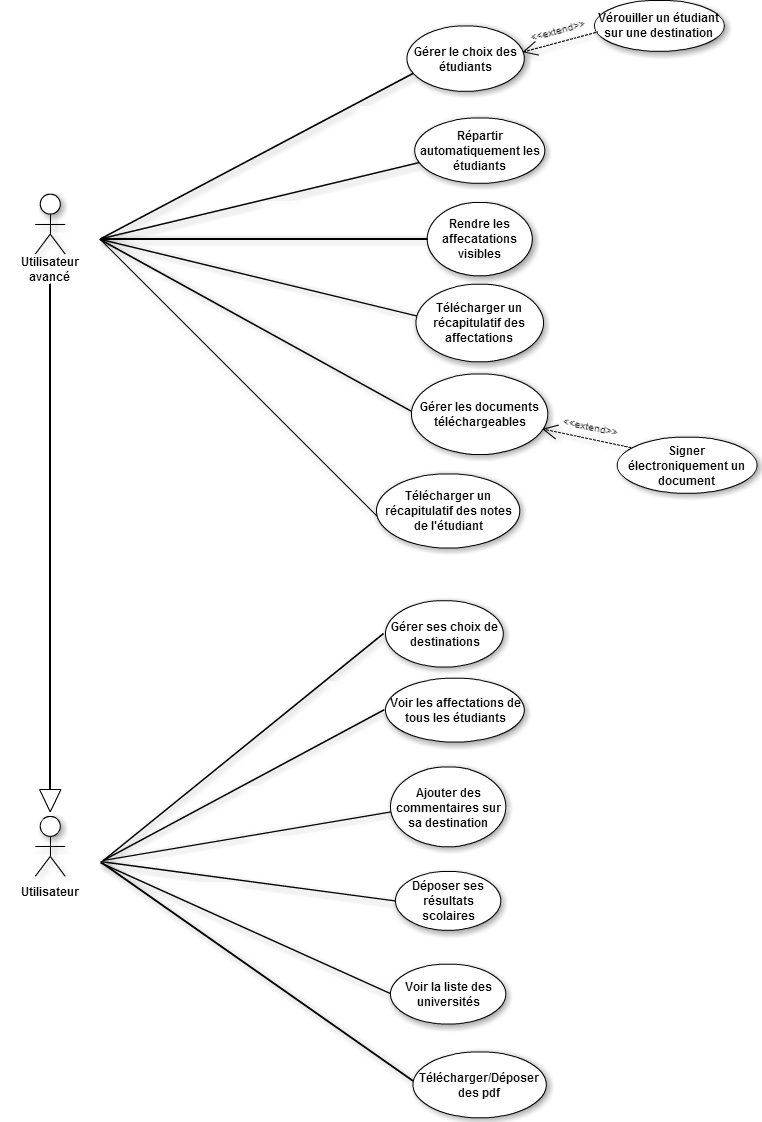
\includegraphics[scale=0.7]{images/useCaseDiagram.png}
	\caption{Diagramme de cas d'utilisation de l'application}
	\label{useCase}
\end{figure}
    
    \chapter{Exigences et aperçu général}
\label{chap::exigences}

\section{Rappel des exigences}

L'application va permettre d'aider les \ris à simplifier la gestion des mobilités des étudiants. L'affectation et le suivi des mobilités sont séparés en trois phases.

\bigbreak

La première correspond, pour les étudiants (ou élèves dans la rapport), à la recherche de l'université de destination et au choix de leurs \voe. Ils doivent donc pouvoir accéder à la liste des écoles. Une liste de commentaires des élèves déjà partis vers ces destinations doit également être présente.

Les \ris peuvent gérer les étudiants, les écoles partenaires, les \voe des étudiants et enfin leur affectation. Les affectations peuvent être effectuées de façon manuelle, ou de façon automatique à l'aide d'un algorithme qui pourra être choisi. Lorsque chaque étudiant a une école qui lui est affectée, la deuxième phase commence.
\bigbreak

Certains documents sont nécessaires pour la mobilité. Ils devront être accessibles en téléchargement, et une génération de façon automatique peut être envisagée. Les \ris et membres du SRI (Service Relations Internationales) doivent pouvoir récupérer ces fichiers. Ils disposeront donc de certaines vues en commun avec les \ris, mais ne pourront pas valider les affectations des étudiants. Enfin, les documents devront être signés de façon électronique. La figure \ref{fig::diffRI-SRI} ci-dessous récapitule les rôles des \ris et des membres du SRI.

\begin{figure}[H]
	\centering
	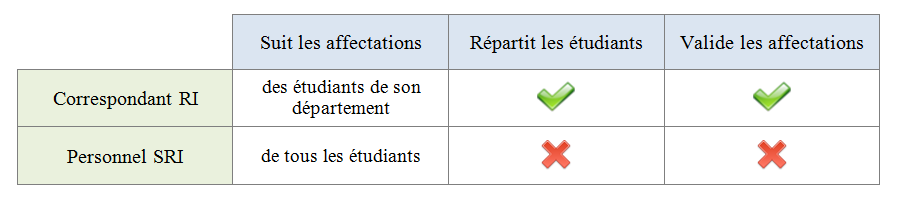
\includegraphics[scale=0.4]{roleRI-SRI.png}
	\caption{Page d'accueil pour les étudiants dans l'étape 1}
	\label{fig::diffRI-SRI}
\end{figure}
\bigbreak

La troisième et dernière phase correspond au suivi des mobilités après le départ des étudiants. Le contrat de mobilité doit pouvoir être modifié par l'élève, et les \ris doivent en être notifiés. Ils pourront ensuite valider le nouveau contrat. A la fin de la mobilité, l'étudiant pourra entrer ses notes sur le site pour le jury de fin d'année. Il pourra également laisser un commentaire sur l'université pour aiguiller les étudiants intéressés. La demande de génération de fiches de jury pourra être demandée par les \ris.

\section{Vue globale de l'application}

\begin{figure}[H]
    \centering
    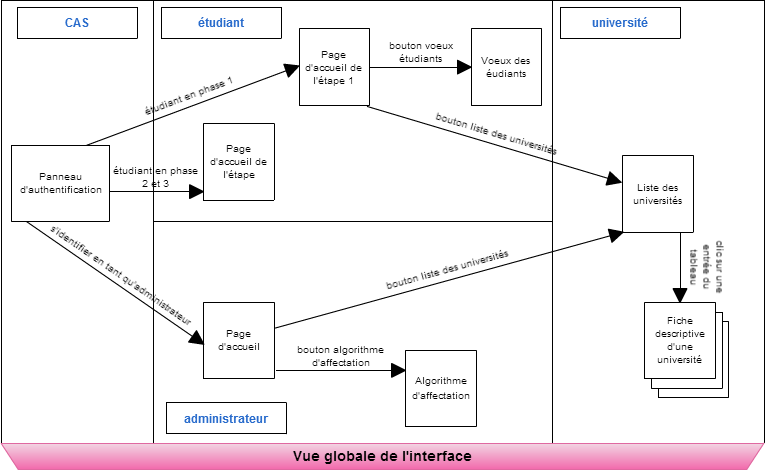
\includegraphics[angle=90,scale=0.7]{Annexe/vue_globale.png}
    \caption{Vue globale de l'interface utilisateur}
    \label{fig::vue_glob}
\end{figure}

	
	
	\chapter{Le projet}
	 Lors de leur 4\ieme{} année d'étude, les étudiants de l'INSA de Rennes doivent réaliser un projet. Notre groupe a choisi %lol
	  le sujet \og Système de gestion informatisé des mobilités \fg. Nous allons donc développer une application facilitant le traitement des étudiants et de réduire la perte de papier due aux nombreuses impressions nécessaires.

		\section{Page d'accueil des étudiants à l'étape 1}

Ceci est la page d'entrée du site pour les élèves.\\
Une fois identifiés via le CAS, ils sont dirigés vers une page qui est propre à chaque élève et qui se modifie selon ses choix.
Sur cette page est présent :
\bigbreak
Un tableau représentant les vœux de l'élèves sous forme d'une liste d'universités.
Chaque lignes du tableau correspond à une université, une ligne du tableau est composé de plusieurs champs qui donnent des informations sur l'université correspondante (comme le pays, la ville etc).
De plus chaque université est un lien vers une "Fiche université" de cette université. Cette fiche donnera toutes les informations nécessaires sur cette université ainsi que les commentaires laissés par les autres élèves des années précédentes.
Le tableau de vœux possède des boutons pour effectuer les actions basiques comme ajouter, supprimer ou modifier ses vœux. Il y a également un bouton pour valider nos choix d'universités et informer que les correspondants RI que cette liste est définitive. La réorganisation des vœux est néanmoins possible après validation de l'élève tant que le correspondant RI n'a pas fixé les vœux.
\bigbreak
Un bouton redirigeant vers "Liste des Universités" (cf section \ref{sec::list_univ}) permettant d'accéder à la liste de toutes les universités.
\bigbreak
Un bouton redirigeant vers "Vœux des Étudiants" permettant d'accéder aux vœux des autres étudiants.

		\section{Page d'accueil des étudiants à l'étape 2}



\begin{figure}[H]
	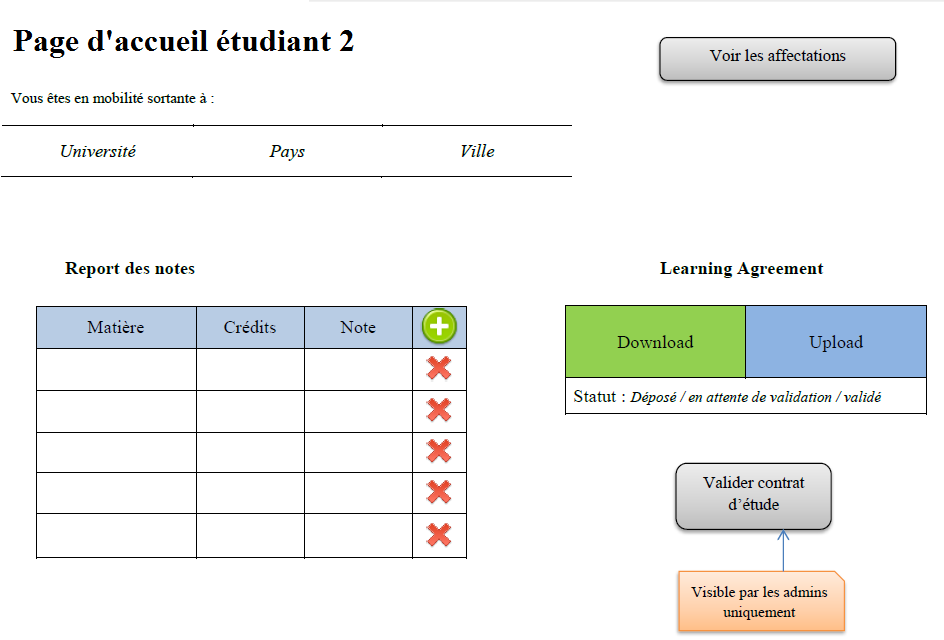
\includegraphics[scale=0.6]{Etudiant/HPS2.PNG}
	\caption{Page d'accueil pour les étudiants dans l'étape 2}
\end{figure}


Cette page est la nouvelle page d'accueil du site une fois l'étape 1 validée.
Elle est comme précédemment propre à chaque étudiant suivant sa destination. De nouvelles informations sont présentes ici.
On peut donc voir ici la destination assignée à l'étudiant en question, avec un lien vers sa "Fiche Université"(cf section \ref{sec::sheet_univ}).

L'élève peut accéder aux vœux des autres étudiants via un bouton "Vœux des Étudiants" (cf section \ref{sec::stud_wish}).
C'est sur cette page qu'est présente la gestion du téléchargement et du dépôt du Learning Agreement, avec un bouton pour télécharger un exemplaire vierge et un bouton pour déposer le document rempli.

Celui-ci est ensuite en attente de validation par le correspondant RI. On peut suivre ici les étapes de validation du Learning Agreement (à déposer, en attente de validation, validé).


\bigbreak

On pourra également trouver un tableau des matières choisies par l'élève qui seront validées par le correspondant RI dans le Learning Agreement.

\subsection{Admin}

L'administrateur (le correspondant RI) peut accéder à cette page avec des fonctionnalités supplémentaires.
Il peut supprimer ou valider/fixer les vœux de l'étudiant manuellement sur cette page (l'étudiant n'interviendra pas dans l'algorithme de sélection).

Le correspondant RI peut valider ici le Learning Agreement et les matières pour un étudiant en particulier.

		\section{Page d'accueil des étudiants à l'étape 3}
C'est la page d'accueil une fois l'étape 2 terminée.

Elle est très proche de celle de l'étape 2. Cependant l'étudiant peut déposer pour cette étape un commentaire sur l'université où il a effectué sa mobilité. Ce commentaire sera accessible par tous les étudiants dans la "Fiche Université" de la destination en question.
		\section{Vœux des Étudiants}
\label{sec::stud_wish}
<<<<<<< HEAD

\begin{figure}[H]
	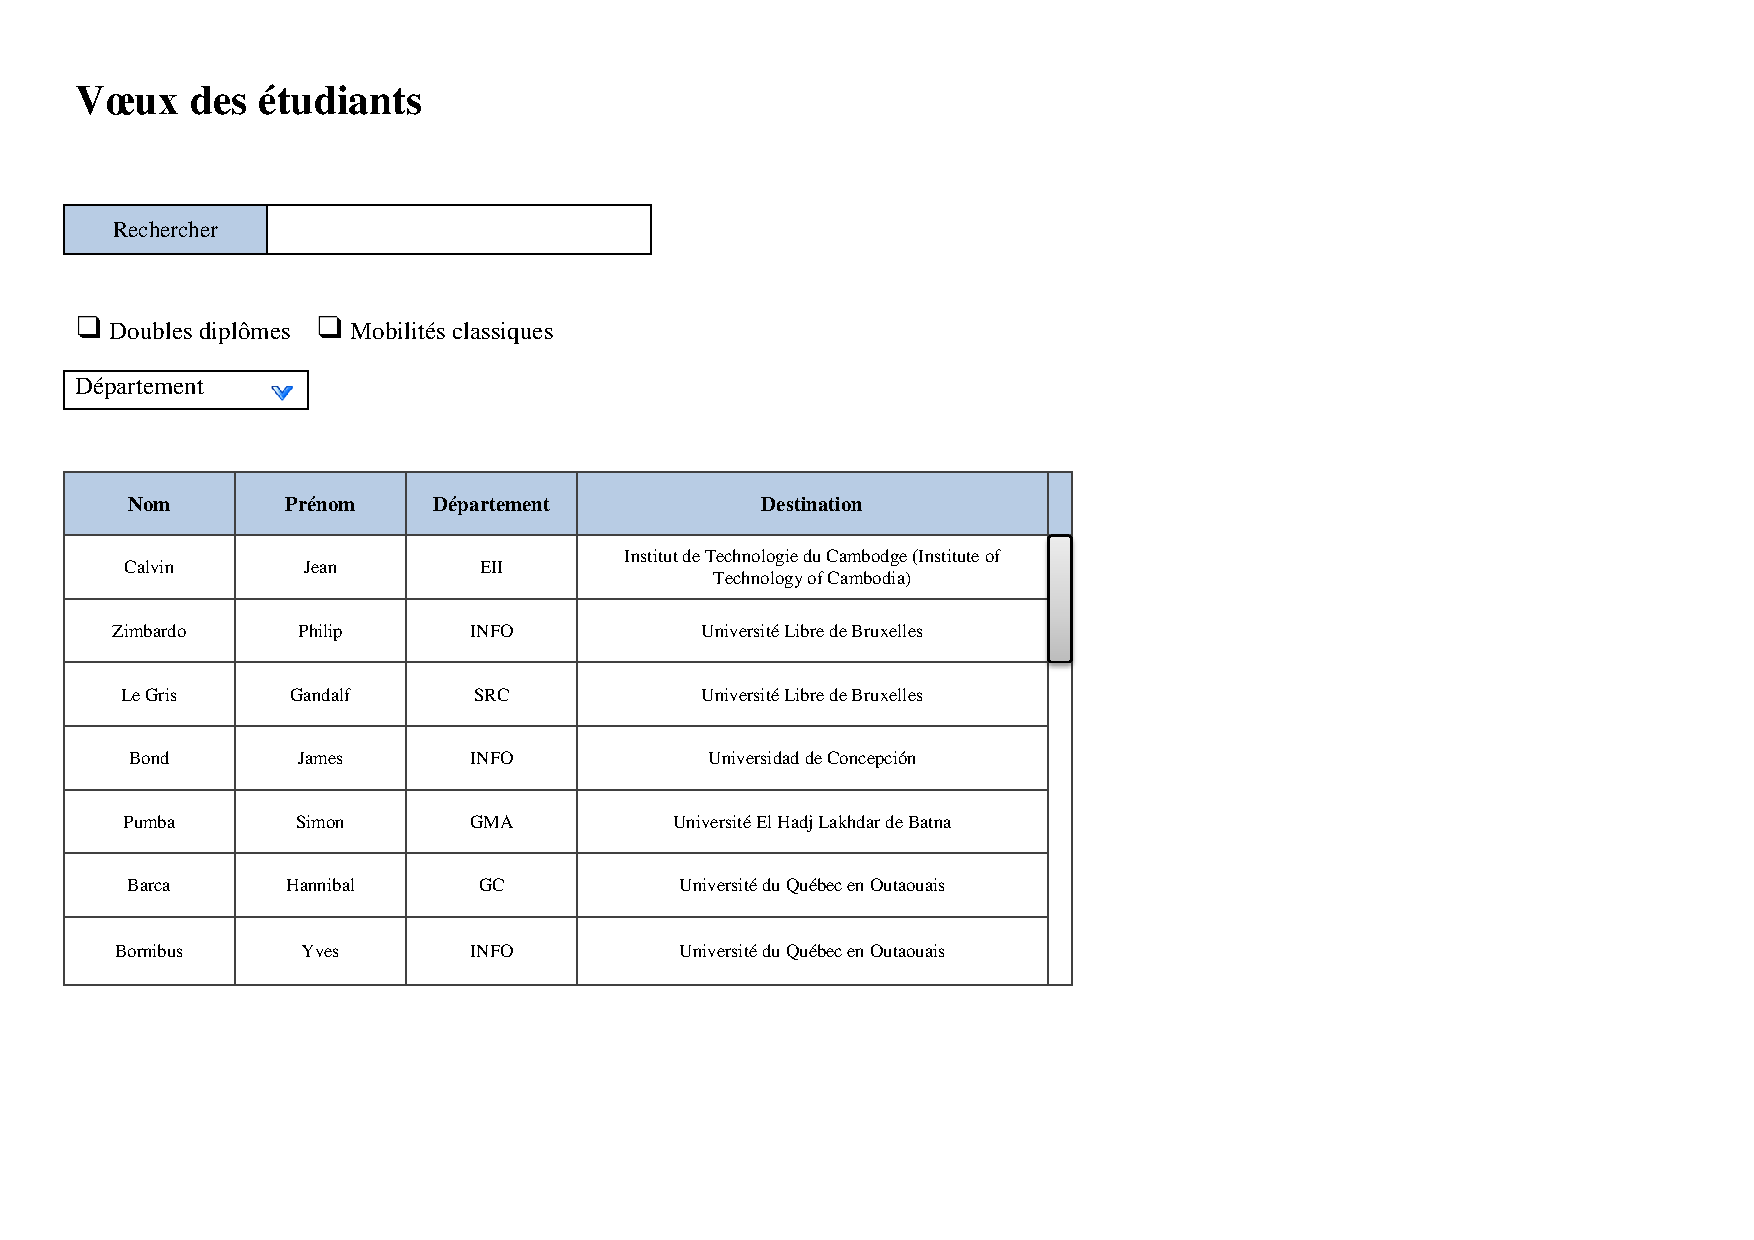
\includegraphics[scale=0.8]{Etudiant/VoeuxEtudiants.pdf}
	\caption{Page des vœux de tous les étudiants}
\end{figure}

Cette page permet d'avoir accès aux vœux de tous les étudiants.\\
On peut filtrer cette liste avec un système de checkbox et de champs de recherche. On peut par exemple soit directement taper le nom de l'élève dans le champs de recherche ou alors avoir accès aux étudiants partant en double diplôme en cochant la case double diplôme.\\
De plus chaque étudiant dans le tableau est un lien vers sa page d'accueil en lecture seule (pour empêcher quiconque de modifier les vœux des autres étudiants)
=======
Cette page permet d'avoir accès aux vœux de tous les étudiants.

On peut filtrer cette liste avec un système de checkbox et de champs de recherche. On peut, par exemple, soit directement taper le nom de l'élève dans le champs de recherche ou bien avoir accès aux étudiants partant en double diplôme en cochant la case correspondante.

De plus chaque étudiant dans le tableau est un lien vers sa page d'accueil en lecture seule (afin empêcher quiconque de modifier les vœux des autres étudiants).
>>>>>>> origin/master

			
	
	\chapter{Le projet}
	 Lors de leur 4\ieme{} année d'étude, les étudiants de l'INSA de Rennes doivent réaliser un projet. Notre groupe a choisi %lol
	  le sujet \og Système de gestion informatisé des mobilités \fg. Nous allons donc développer une application facilitant le traitement des étudiants et de réduire la perte de papier due aux nombreuses impressions nécessaires.

	 	\section{Page d'accueil des administrateurs}
\label{sec::home_admin}

\begin{figure}[H]
	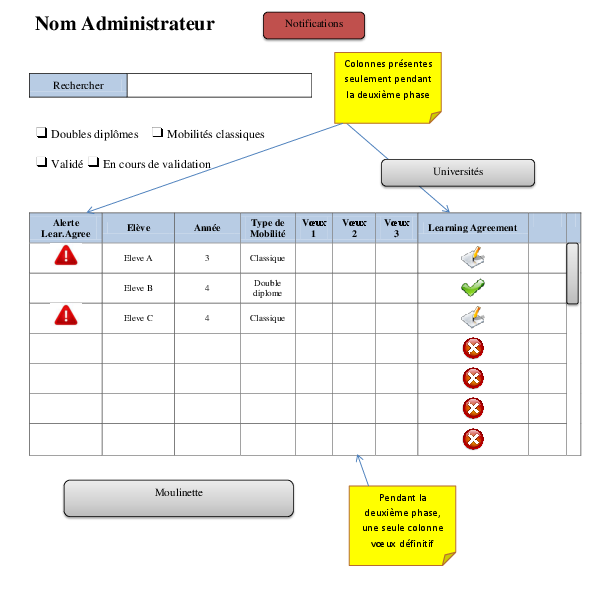
\includegraphics[scale=0.7]{Admin/HomeAd.png}
	\caption{Page d'accueil des administrateurs}
	\label{fig::hpa1}
\end{figure}

La figure \ref{fig::hpa1} représente la page sur laquelle un administrateur arrive après sa connexion au CAS. Cette page va servir à gérer les vœux des élèves lors de la première phase mais aussi les documents déposés par les élèves lors de la seconde.

Le principal élément de cette page est un tableau regroupant:
\begin{itemize}
 	\item le nom de l'élève ;
 	\item l'année de l'élève ;
 	\item si l'élève souhaite une mobilité classique ou double diplôme ;
 	\item une case précisant si les vœux de l'élève sont définitifs ou non (en phase 1) ;
 	\item une case précisant l'état de l'élève (Learning Agreement en attente, en cours de validation, validé) (en phase 2) ;
 	\item la liste des \voe de l'élève (en phase 1) ;
 	\item le \voe de l'élève (en phase 2) ;
 	\item une case d'alerte prévenant du dépôt d'un Learning Agreement à valider.
 \end{itemize}
 
 \bigbreak
 
Dans le tableau, le nom des élèves est un lien vers leur page d'accueil sur laquelle l'administrateur peut être redirigé. Cela lui permet de modifier les vœux d'un élève.

Les \voe de l'élèves sont aussi des liens ramenant sur la page des universités en mode administrateur. Cela permet notamment d'ajouter de nouvelles universités ou de mettre des commentaires professeurs sur une université existante.

Au dessus du tableau, l'administrateur pourra utiliser une barre de recherche par mot-clé ainsi que des filtres (Learning Agreement en attente de validation, Learning Agreement validé, double diplôme, mobilité classique, année d'étude de l'élève).

\bigbreak

Également présente en haut de la page, une case de notification des Learning Agreement récemment déposés. Le fait de cliquer sur cette case nous emmène au tableau sur lequel un filtre est ajouté pour ne voir que les élèves concernés.

\bigbreak

On trouvera aussi un lien permettant à l'administrateur d'accéder à la liste des universités mais en mode administrateur.

\bigbreak

Enfin l'administrateur dispose d'un lien lui permettant d'accéder à l'algorithme d'affectation. Il permet, à la fin de la phase de vœux, de faire la répartition des destinations pour les élèves.
	 	\section{Algorithme d'affectation}
\label{sec::moulinette}

\begin{figure}[H]
	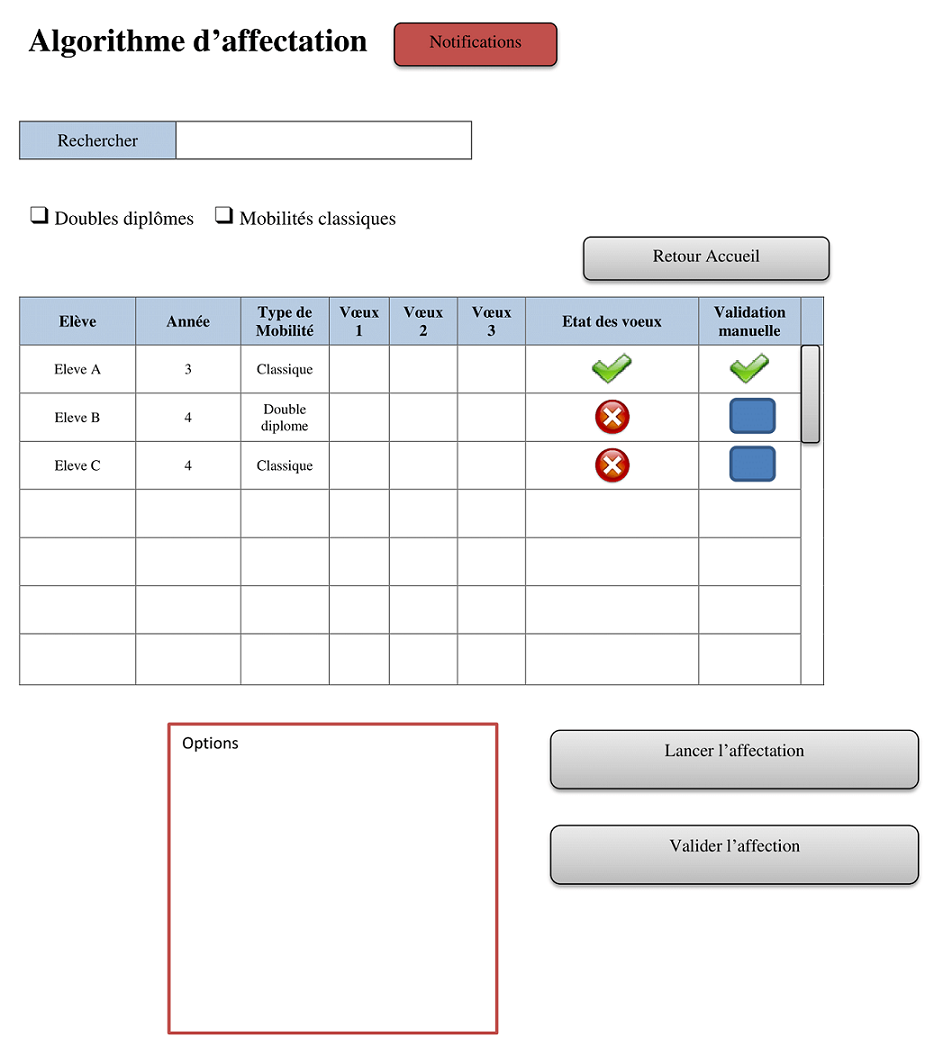
\includegraphics[scale=0.7]{Admin/Moul.png}
	\caption{Page de gestion de l'algorithme d'affectation}
	\label{fig::moulinette}
\end{figure}

La figure \ref{fig::moulinette} présente la page sur laquelle se trouve un tableau récapitulant les vœux définitifs des élèves, après la fin des choix de vœux (phase 1). Ce tableau comprend donc la liste des élèves, leur année, la liste des vœux, le type de mobilité choisie (double diplôme, mobilité classique), leur état (validé, à validé).

Encore présent sur ce tableau; une zone de recherche par mot clé ainsi que plusieurs filtres (années, universités, type de mobilité...).

\bigbreak

L'administrateur peut, sur cette page, gérer les paramètres de l'algorithme avant de le lancer (ajout de paramètres particuliers modifiant l'ordre d'attribution des vœux, en plus des notes).

\bigbreak

Il est aussi possible à l'administrateur de valider les vœux d'un élève manuellement. Cela fait sortir cet élève de la liste des élèves concernés par l'algorithme (il apparaitra toujours dans la liste des élèves mais son état deviendra "validé" et il ne sera pas pris en compte par l'algorithme).

\bigbreak

Enfin, un bouton permettant de lancer l'algorithme d'attribution des vœux. Lorsque l'algorithme est terminé, la phase 1 est finie et la phase 2 est lancée. Cela signifie que les différentes vues deviendrons celles de la phase 2.
	 	\section{Page d'accueil de l'étudiant}

L'administrateur (le correspondant RI) peut accéder à la page d'accueil de l'étudiant (cf \ref{fig::hps1}) avec des fonctionnalités supplémentaires.
Il peut supprimer ou valider/fixer les vœux de l'étudiant manuellement sur cette page (l'étudiant n'interviendra pas dans l'algorithme de sélection).

Le correspondant RI peut valider ici le Learning Agreement et les matières pour un étudiant en particulier.
	 	\section{Page d'accueil SRI}

Tout comme les administrateurs, les membres du SRI ont accès à une interface spéciale. Celle-ci est semblable à celle des administrateurs, à quelques différences près:
\begin{itemize}
 	\item le tableau d'élèves présents sur leur page d'accueil regroupe tout les élèves des différents départements ;
 	\item à ce titre, le tableau contient une colonne supplémentaire avec le département de l'élève ;
 	\item Le SRI ne possède pas d'accès à l'algorithme d'affectation ;
 	\item Le SRI ne peux pas valider ou modifier les vœux d'un élève.
 \end{itemize}
	 
	 
	\chapter{Le projet}
	 Lors de leur 4\ieme{} année d'étude, les étudiants de l'INSA de Rennes doivent réaliser un projet. Notre groupe a choisi %lol
	  le sujet \og Système de gestion informatisé des mobilités \fg. Nous allons donc développer une application facilitant le traitement des étudiants et de réduire la perte de papier due aux nombreuses impressions nécessaires.

		\section{Tableau des destinations}
\label{sec::list_univ}

\begin{figure}[h!]
	\centering
	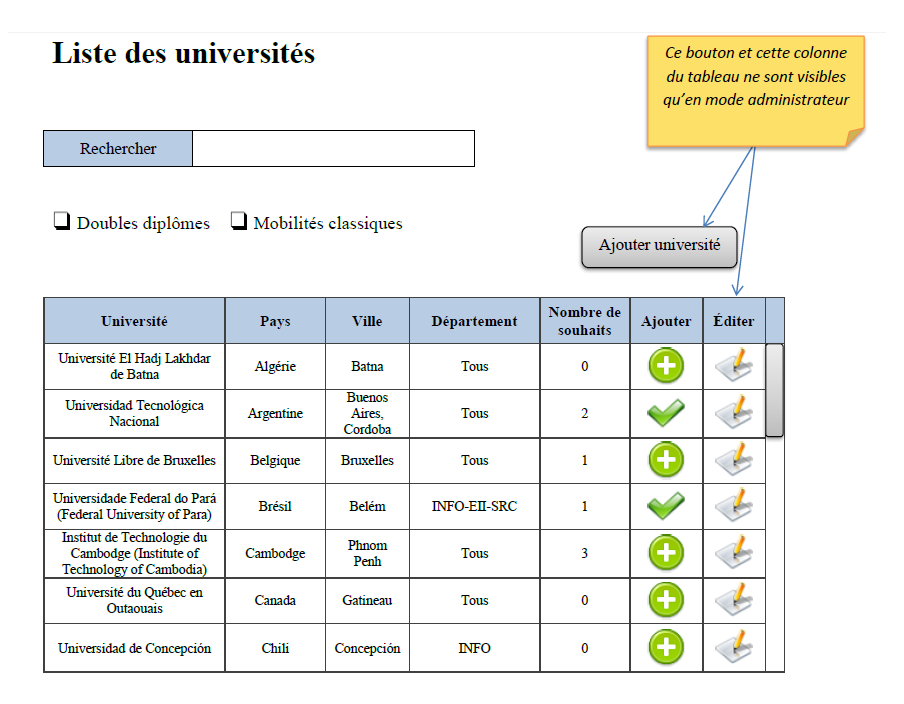
\includegraphics[scale=0.7]{Universites/listeUnivs.png}
	\caption{Tableau contenant la liste des universités}
	\label{fig::list_uni}
\end{figure}



Une page (cf. figure \ref{fig::list_uni}) de notre application servira à renseigner la liste des destinations accessibles aux étudiants.
Les universités seront regroupées dans un tableau, pour lequel chaque ligne présentera les informations suivantes :
 \begin{itemize}
 	\item le nom de l'université partenaire ;
 	\item le pays dans laquelle elle se trouve ;
 	\item les départements pour lesquels cette destination est disponible ;
 	\item s'il s'agit d'un double diplôme ;
 	\item le nombres d'étudiants ayant fait ce vœux du/des département(s) sélectionné(s) ;
 	\item un bouton, à disposition des étudiants, pour ajouter cette destination à leur liste de vœux.
 \end{itemize}
 
Pour faciliter son parcours, une barre de recherche fonctionnant par mot-clef sera disponible au dessus du tableau. Un utilisateur pourra aussi sélectionner des filtres en haut du tableau. Il pourra filtrer par département ou pays en sélectionnant un choix parmi un menu déroulant. L'utilisateur pourra aussi cocher les cases \og Doubles diplômes\fg{} ou \og Mobilité classique \fg{}. Pour accéder à la fiche d'une université, il suffira de cliquer sur la ligne correspondante (sauf pour le bouton \og Ajouter \fg{}). Si une destination figure déjà parmi les vœux de l'étudiant, la case \og Ajouter \fg{} le figurera avec une icône différente.

Il y a dissociation entre les doubles diplômes et les mobilités classiques. Si une destination propose les deux, un étudiant pourrait demander deux fois la destination, une pour chaque type de mobilité. Ce choix se fera dans une fenêtre apparaissant en cliquant sur "Ajout". 
Les administrateurs auront aussi à disposition des boutons pour éditer chaque destination, dont un bouton pour définir si le partenariat est actif ou non. Un partenariat inactif ne sera pas visible pour les étudiants.

L'édition d'une entrée du tableau les reconduira vers la fiche où se trouvent toutes les informations sur la destination.
Les administrateurs pourront aussi supprimer une université du tableau s'ils le souhaitent.

Les administrateurs pourront ajouter des universités au tableau via un bouton. Ils devront alors remplir une fiche descriptive de la nouvelle destination. L'université sera ajoutée au tableau une fois la fiche validée. De plus, le bouton \og Ajouter université \fg{} leur permettra de télécharger (upload) la liste des universités au format CSV.
 

		 \section{Fiche de destination}
 \label{sec::sheet_univ}
 
 \begin{figure}[H]
 	\centerline{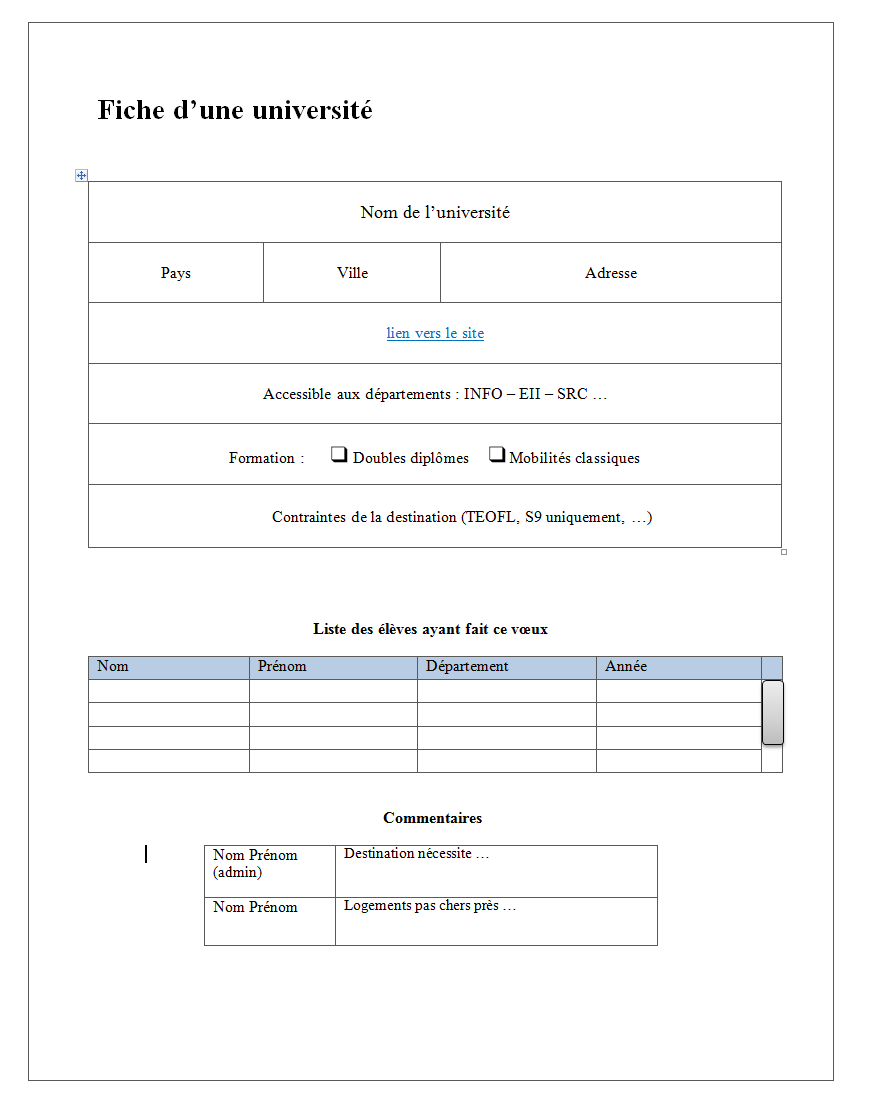
\includegraphics[scale=0.5]{Universites/ficheUniv.png}}
 	\caption{Exemple de fiche descriptive d'un établissement partenaire}
 \end{figure}
 
 Chaque université partenaire disposera d'une fiche où figureront les informations complémentaires au tableau.
 On y trouvera notamment toutes les informations présentes dans le tableau ainsi que :
 \begin{itemize}
 	\item un lien vers le site de l'université
 	\item si la destination propose un double diplôme
 	\item (facultatifs) certains pré requis de la destination, comme le TOEFL par exemple, ou si la destination n'est disponible qu'en S9...
 	\item les commentaires des responsables RI et des élèves déjà partis sur cette destination
 	\item la liste des étudiants ayant déjà choisis ce vœux
 \end{itemize}
 

 
 Les admins pourront aussi éditer ou supprimer un partenariat directement depuis la fiche.
		
	
	\chapter{Le projet}
	 Lors de leur 4\ieme{} année d'étude, les étudiants de l'INSA de Rennes doivent réaliser un projet. Notre groupe a choisi %lol
	  le sujet \og Système de gestion informatisé des mobilités \fg. Nous allons donc développer une application facilitant le traitement des étudiants et de réduire la perte de papier due aux nombreuses impressions nécessaires.

		Le modèle de notre application sera constitué d'une base de donnée \sql. Nous avons défini son architecture tel que suit:

%image du truc, un pti retro engeenering avec mes entity comme Jeannot avais fait avec le truc à Nico?
TO DOOOOOOOO!!!!!! (comme la panthère rose : 

To Do,

To Do,

To Do  to do  to do, to do  to doooo


\subsection{Les modules}
Plusieurs informations importantes sont présentes dans cette base. Chacune de ces nœuds formera un bundle : 
\begin{itemize}
\item les utilisateurs ;
\item les universités ;
\item les fichiers ;
\item les affectations.
\end{itemize}
Un dernier bundle contiendra les vues principales et diverses.

\subsection{Utilisateur}

Nous utiliserons le bundle FOSUser qui contient des méthodes et une structure de donnée développée pour gérer les utilisateurs.
Les utilisateurs possèdent un état qui défini leur avancement dans la procédure d'affectation. C'est lui qui déterminera la vue d'accueil qui s'affichera pour l'étudiant. 
Chaque année, après une action d'un administrateur, les étudiants seront chargés depuis le LDAP pour mettre à jour la base de données et définir si un étudiant a redoublé ou non.
Ces utilisateurs sont assurés d'être uniques pour toujours grâce à leur id étudiant.

\subsection{Universités}

Les universités possèdent des spécificités qui serviront pour les tris dans les vues (TOEFL, Europe, etc).
Elle sont associées à une classe Place qui permet de définir le nombre de places disponibles pour un département à un semestre donné (ou double diplôme). Une université pouvant proposer plusieurs types de mobilité, cette classe est séparée.
Il existera dans le futur une classe pour définir les informations sur la page de chaque université, mais ne sachant pas encore exactement les champs nécessaire, nous n'avons pas encore implémenté la classe.

\subsection{Fichiers}

Il y a deux types de fichiers à gérer, les fichiers vierges mis à disposition des élèves et ceux qui sont complétés.

Certains fichiers vierges peuvent être associé à des spécificités (Learning Agreement pour les destinations Erasmus par exemple). Ils seront donc proposés par défaut lors de l'affectation à une université.
Les fichier à compléter sont liés à l'année et au département pour permettre de les garder en base un certain temps et les trier relativement facilement.

\subsection{Affectation}

Dans cette partie nous trouvons les \voe et le placement d'un candidat. Les voeux sont lié au département et à l'année en plus de l'utilisateur pour permettre là aussi un historique.
Le placement est l'endroit définitif où l'étudiant est affecté. Il possède aussi la problématique de l'historique.

\subsection{Généralité}

Il reste l'année et les département. 
Il existera un département \textbf{ALL} pour permettre de définir un nombre de places diponibles commun à toute l'INSA, et non pas à un seul département.


% Diagramme d'architecture logicielle

	 
	\chapter*{Conclusion}
\addcontentsline{toc}{chapter}{Conclusion}	

Au terme de cette étape, nous avons défini un premier design de notre application, en expliquant les fonctionnalités offertes aux utilisateurs. 
Les chapitres \ref{chap::etudiants} et \ref{chap::admins} présentent l'interface offerte à chaque type d'utilisateur par notre application. Le chapitre \ref{chap::universites} explique comment les utilisateurs accèderont aux informations sur les universités.
Enfin, le chapitre \ref{chap::archi_logicielle} présente succinctement l'architecture logicielle de notre application.
Nous pouvons aussi présenter une ébauche des vues accessibles, bien que l'apparence même soit sans doute sujette à changement.
\bigbreak
Nous allons désormais travailler à l'implémenter puis tester un premier prototype fonctionnel. Celui-ci répondra à la première étape d'un cycle de départ en mobilité, c'est-à-dire les vœux des étudiants puis leur affectation. L'objectif étant d'avoir à disposition une version incomplète mais fonctionnelle de l'application, pour la tester en situation réelle courant Décembre. 
	
	\appendix
        \chapter*{Annexe}

\begin{figure}[H]
	\centering
	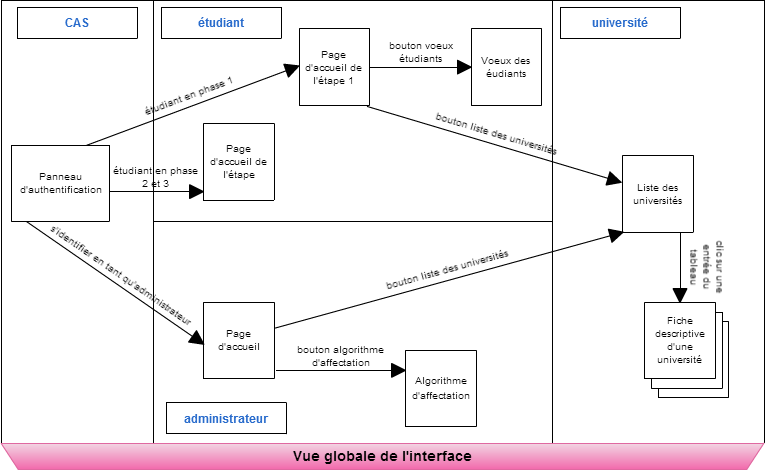
\includegraphics[angle=90,scale=0.7]{Annexe/vue_globale.png}
	\caption{Vue globale de l'interface utilisateur}
	\label{fig::vue_glob}
\end{figure}
\end{document}


